\subsubsection{Funktionsweise}
Wie bereits aus den Definitionen unter Punkt \ref{subsub:def} hervorgeht, hat ein Webcrawler stets ein bestimmtes Ziel, auf welches er hinarbeitet. Um dieses Ziel zu erreichen, durchforstet ein Webcrawler das Internet, indem er von einem oder mehreren Startadressen, sog. \emph{Seeds}, ausgehend, Webseiten aufruft, deren Inhalt herunterlädt, ihn mithilfe von diversen Algorithmen analysiert und dann die Webseite wieder verlässt. Während des Aufrufs der Webseite, filtert sich ein Webcrawler alle weiterführenden Hyperlinks heraus, um sie dann später in einem zweiten Moment aufrufen zu können. Diese Hyperlinks speichert er zusammen mit den Seeds in einer Liste, einer sog. \emph{Queue}\footnote{Das englische Wort \glqq Queue\grqq\space kann ins Deutsche mit dem Wort \emph{Warteschlange} übersetzt werden.}. Die Einträge in dieser Liste werden meist als URLs\footnote{URL steht für \emph{\underline{U}niform \underline{R}esource - \underline{L}ocator} und ist ein eindeutiger Zeiger auf ein Objekt im Internet. https://www.example.org wäre z.B. eine URL.} gespeichert. Diese Liste wird Schritt für Schritt, meist nach dem FIFO-Prinzip\footnote{FIFO steht für \emph{\underline{F}irst \underline{I}n - \underline{F}irst \underline{O}ut} und beschreibt hierbei ein Verfahren, bei welchem das Objekt (in diesem Fall die URL), welches als erstes gespeichert wird (IN), auch als erstes verwendet wird(OUT).} abgearbeitet. So besucht er rekursiv\footnote{\emph{Rekursiv} bedeutet sich selbst definierend und beschreibt in der Informatik einen Sachverhalt, in welchem sich ein Programm, eine Funktion wiederholend selbst aufruft, um eine komplexes Problem auf einfache Operationen herunterzubrechen.} Webseite um Webseite und übermittelt die gewonnenen Informationen an ein zentrales System, beispielsweise einem Server. Alternativ können die gewonnenen Informationen auch direkt im Webcrawler zwischengespeichert und später von Hand ausgelesen werden. Diese Arbeitsweise wird im Flussdiagramm aus Abbildung \ref{fig:arbeitsweise_crawler} nochmals grafisch verdeutlicht.
\begin{figure}[H]
	\centering
	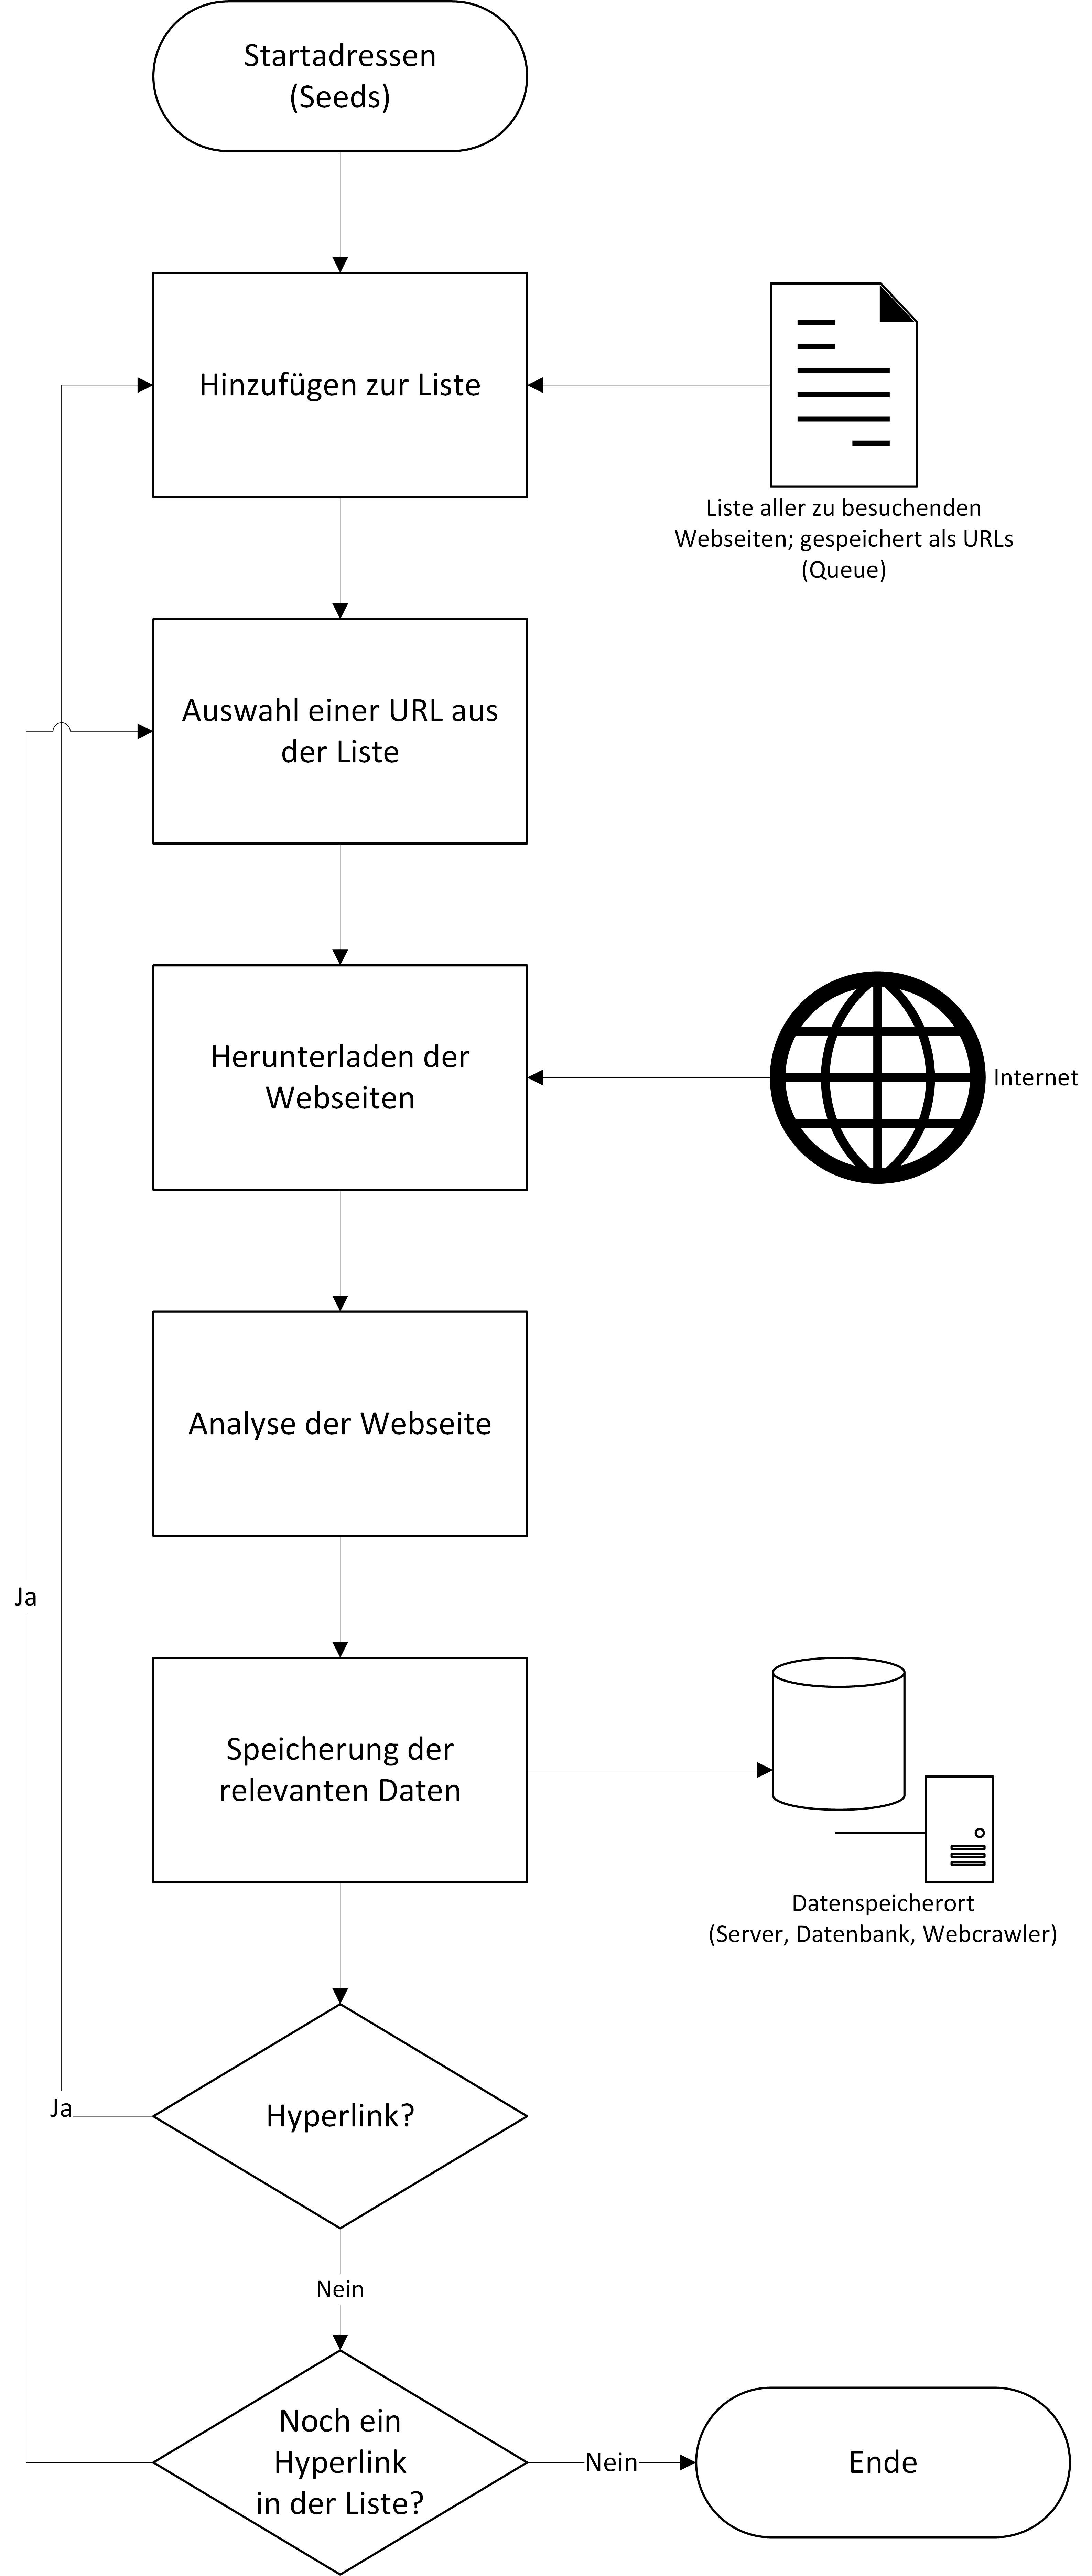
\includegraphics[width=8.45cm]{img/flussdiagramm-ablauf-webcrawler-neu.png}
	\caption{Arbeitsweise eines Webcrawlers}
	\label{fig:arbeitsweise_crawler}
\end{figure}
Da das Internet ein sich stets weiterentwickelndes und wandelndes Medium ist, in welchem sich Webseiten teils im Stundentakt ändern, muss ein Webcrawler gewissen Prinzipien folgen, welche in den folgenden vier Richtlinien aufgelistet sind.\cite[265-267]{ijcsc-web-crawler-overview} Somit kann gewährleistet werden, dass ein Webcrawler ein akzeptables Ergebnis erzielt.
\begin{enumerate}
	\item \textbf{Selection Policy \emph{(Auswahlrichtlinie)}}\newline
	Im Durchschnitt kommen alle zwei Sekunden rund zehn neue Webseiten hinzu\footnote{Messung selbst durchgeführt mit den Daten von internetlivestats.com\cite{zaehler-webseiten}.}. Dass ein Webcrawler nicht alle Webseiten besuchen kann ist somit selbsterklärend. Deshalb liegt es im Interesse des Betreibers eines Webcrawlers, dass dieser gezielt jene Webseiten untersucht, welche eine hohe Chance auf einen für den Betreiber relevanten Inhalt haben. Jeder unnötige Aufruf und jede unnötige Analyse einer Webseite verbraucht Ressourcen. Vor allem die Ressource \emph{Zeit} ist für Webcrawler  besonders wertvoll, denn mit jeder vergangenen Sekunde werden wieder neue Webseiten online gestellt. 
	%TODO: LÖSCHEN
	%Dies führt beispielsweise zu den unfassbaren 1.838.596.056 Webseiten\footcite[Stand Februar 2018:][]{stat-webseiten}, welche aktuell online sind.
	
	\item \textbf{Revisit Policy \emph{(Wiederbesuchsrichtlinie)}}\newline
	Neben den neu ins Netz gestellten Internetseiten, werden die bestehenden Webseiten auch stets aktualisiert. Neue Einträge kommen hinzu, alte werden gelöscht. Eines der besten Beispiele hierfür sind die unzähligen Nachrichtenportale im Internet: Dort werden oft im Minutentakt neue Meldungen, was im Grunde nichts anderes als neuer Inhalt ist, hinzugefügt. All dies sind Einträge, welche sich ein potentiell interessierter Webcrawler erneut holen und analysieren muss. Deshalb müssen Webcrawler abwägen, ob, wann und wie oft sie eine Seite erneut besuchen möchten oder auch müssen.
	%TODO: LÖSCHEN
	%, um ihren aktuellen \glqq Wissensstand\grqq\space auf einer der Webseite angemessenen Aktualität zu halten.
	
	\item \textbf{Politeness Policy \emph{(Höflichkeitsrichtlinie)}}\newline
	Eine Webseite ist heutzutage in wenigen Sekunden komplett geladen, Bilder, Videos oder ähnliche Medien inklusive. Bedenkt man nun, dass GoogleBot\footnote{Mehr zu GoogleBot in Kapitel \ref{subsub:googlebot}.}, ein Webcrawler des Internetgiganten Google, an die zehn Webseiten pro Sekunde\cite{googlebot-anzahl-pro-sekunde} anfragt und man mit einer durchschnittlichen Seitengröße von 3 Megabyte\cite{durch-seitengroesse} rechnen kann, so kommt man auf folgende einfache Gleichung:
	\begin{align*}
		10\ \nicefrac{Webseiten}{Sekunde}\ *\ 60\ Sekunden\ &=\ 600\ \nicefrac{Webseiten}{Minute}\\
		600\ \nicefrac{Webseiten}{Minute}\ *\ 60\ Minuten\ &=\ 36.000\ \nicefrac{Webseiten}{Stunde}\\
		36.000\ \nicefrac{Webseiten}{Stunde}\ *\ 3\ \nicefrac{Megabyte}{Webseite}\ &=\ 108.000\ \nicefrac{Megabyte}{Stunde} 
	\end{align*}
	Wie man hier erkennen kann, ist ein Webcrawler in der Lage, in kürzester Zeit eine Unmenge an Datenverkehr zu produzieren und somit wertvolle Bandbreite eines Webservers zu verschwenden. Da die Performance einer Webseite zu einem großen Teil auch von der Antwortzeit und der Auslastung des Webservers abhängt, kann durch einen Missbrauch eines Webcrawlers die Performance einer Webseite stark leiden. Während Webcrawler mit einem guten Zweck versuchen die Ressourcen des Webservers so wenig wie möglich in Anspruch zu nehmen, sind schadhafte, oder einfach nur schlecht geschriebene Webcrawler in der Lage ganze Server lahm zu legen und somit einen großen Schaden anzurichten.
	\item \textbf{Parallelization Policy \emph{(Parallelisierungsrichtlinie)}}\newline
	Da ein Webcrawler unter Umständen eine große Zeitspanne damit beschäftigt ist, auf die Antwort des Webservers zu warten, ist es natürlich selbstverständlich, dass man versucht die einem zur Verfügung stehenden Ressourcen bestmöglich auszunutzen. Ein Ansatz hierfür ist es, einen Webcrawler parallel ablaufen zu lassen. Hierfür müssen sich diese jedoch untereinander absprechen, damit zwei parallelisierte Webcrawler nicht dieselbe Webseite analysieren und somit erneut wertvolle Ressourcen verschwenden.
\end{enumerate}
Das Ziel eines jeden Entwicklers und Betreibers von Webcrawlern sollte es sein, diese vier Richtlinien zu respektieren und zu gewährleisten.\\
Diese Richtlinien werden jedoch des öfteren verletzt. Unerfahrene Programmierer können durch Programmierfehler diese Richtlinien unbewusst missachten und damit einen großen Schaden anrichten. Meistens werden diese Richtlinien jedoch bewusst verletzt, um in möglichst kurzer Zeit eine große Anzahl an Informationen zu gewinnen. Webcrawler, die diese Richtlinien bewusst verletzen, haben meist böse Absichten und sollten von den Webseiten ferngehalten werden.
\label{subsub:funk}








%\begin{figure}
%	\centering
%	\includegraphics[width=6cm]{flower}
%	\caption{Ein Beispiel.}
%	\label{fig:flower}
%\end{figure}






